\section{Implementation and Performance Evaluation}
\subsection{Software and reproducibility}
The implementation targets Python 3.11 and uses SimPy for event scheduling, PyTorch for learning, and
NumPy, pandas, Matplotlib and PyYAML for workload preparation and analysis.
For the six-policy comparison, we matched task identifiers and arrival
timestamps, verified the trace and topology fingerprints, and checked
that training, validation and evaluation noise seeds were disjoint.
The resulting dataset contains 52,110 task outcomes and 90 replay
summaries. A 20-task pilot with each algorithm verified that all
policies ran on the same reference configuration.

\subsection{Dataset and workload construction}
Alibaba Cluster Trace 2017 records a 24-hour period from part of a
production cluster that runs batch jobs and online services
\cite{alibaba2017}. We use the batch task and instance tables. The task
table supplies creation time and the job and task identifiers. The
instance table supplies start and finish timestamps and average CPU
use in cores. We join the two tables by job and task identifiers.

We retain completed tasks belonging to single-task jobs with at least
one valid completed instance. For task $i$, the work in million
instructions (MI) is derived as
\begin{equation}
w_i=\frac{c_{\rm ref}}{|\mathcal I_i|}
\sum_{j\in\mathcal I_i}(t^{\rm end}_j-t^{\rm start}_j)u_j,
\end{equation}
where $\mathcal I_i$ contains valid completed instances, $u_j$ is
average CPU use and $c_{\rm ref}=1000$ MIPS per core is a modeling
constant. The average represents a typical instance. Summing across
parallel instances would map their combined work onto one sequential
service. The filter retains 2,891 of 80,553 task records. In the
separate instance table, 147,849 records are flagged for malformed
fields or invalid completed-instance measurements.

The accepted tasks are sorted by arrival and split chronologically
into 1,734 training, 578 validation and 579 test tasks.
Fig.~\ref{fig:workload} shows the compute-demand quantiles by split.

\begin{figure}[t]
\centering
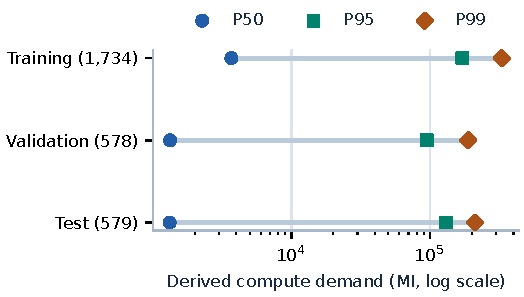
\includegraphics[width=\columnwidth]{figures/workload_quantiles.pdf}
\caption{Compute demand after trace adaptation. Each row reports
the median, P95 and P99 for one chronological split.}
\label{fig:workload}
\end{figure}

The accepted test tasks span 9,753 trace seconds. Their median work is
1,320 MI and their P95 work is 131,057 MI. The six largest tasks account
for 14.5\% of the test workload. A P95-sized task takes about 6.55 s
of nominal service even at 20,000 MIPS. A single worker can therefore
remain occupied while several smaller jobs arrive.

The evaluation uses the best-tier-calibrated deadline rule with a one-second
floor and validation-calibrated arrival compression
$0.12793575549650835$. Payload sizes, device assignment, device battery and
radio state, wireless bandwidth and propagation, edge/cloud capacities, and
relative deadlines are simulator assumptions. Input size is assigned
reproducibly per task using a lognormal distribution with median 1 MB,
log-scale standard deviation 1 and a cap of 50 MB. The result returned
to the device is 0.1 MB. Tasks are assigned round-robin to 24 devices
with fixed edge associations. The test median interarrival time changes
from 10 s in the trace to 1.28 s after compression. The dataset
therefore supplies workload timing and compute demand, while the
simulator defines the mobile network and deadline regime.

\subsection{Matched evaluation protocol}

The primary comparison uses 579 tasks on the reference topology: 24 devices,
three edges, and one cloud worker. Random, Greedy/FIFO, and Greedy/EDF are
fixed baselines evaluated with noise seeds 10001--10005. Centralized DQN uses
the five standard-DQN checkpoints from training seeds 42--46, observes global
state, and uses fixed EDF cloud dispatch. Hierarchical DQN and hierarchical
Double DQN use the ten frequent-feedback bundles at the same five training
seeds; their cloud rules are learned. For learned policies, five noise runs
are averaged within each training seed, then the mean and sample standard
deviation are computed across five training-seed means. Baseline deviations
are across the five noise seeds. P95 is computed per replay before
aggregation, so these two SDs describe different variation sources.

\begin{table}[t]
\centering
\caption{Reference simulation and training settings.}
\label{tab:settings}
\small
\begin{tabular}{@{}p{.31\columnwidth}p{.63\columnwidth}@{}}
\toprule
Parameter & Setting \\
\midrule
Compute capacity & Device 800/1,000/1,200 MIPS, edge
5,000/6,250/7,500 MIPS, cloud 20,000 MIPS \\
Device--edge link & 100 Mb/s, 10 ms propagation \\
Edge--cloud link & 1,000 Mb/s, 40 ms propagation \\
Timing noise & Bandwidth and service perturbations of up to 10\% \\
Relative deadline & $\max\{1,\,0.9w/20000+0.5\}$ s, with $w$ in MI \\
Training & Up to 1,000 episodes of 100 tasks, nine training topologies \\
Exploration & Linear from 0.90 to 0.05 over the first 75\% of the budget \\
Validation & 578 tasks, five noise seeds, every 25 episodes \\
\bottomrule
\end{tabular}
\end{table}

Table~\ref{tab:settings} lists the main settings. Checkpoint selection
maximizes validation deadline success and uses lower P95 to break ties.
Training stops early after eight validation checks without improvement
for both learners. For the test, the original deadline
formula stays fixed when changing topology.

\subsection{Matched six-policy comparison}
Table~\ref{tab:matched} is the primary result. Device energy is reported in
joules per task. Reported means and standard deviations summarize the
observed replays.

\begin{table}[t]
\centering
\caption{Matched reference-topology comparison. Means $\pm$ SD; P95 is per
replay before aggregation.}
\label{tab:matched}
\scriptsize
\resizebox{\columnwidth}{!}{%
\begin{tabular}{lrrr}
\toprule
Policy & Deadline success (\%) & P95 latency (s) & Device energy (J/task)\\
\midrule
Random & $49.57\pm0.95$ & $137.96\pm16.46$ & $10.480\pm0.720$\\
Greedy/FIFO & $75.79\pm0.78$ & $13.62\pm0.49$ & $0.211\pm0.001$\\
Greedy/EDF & $75.89\pm0.86$ & $12.95\pm0.43$ & $0.211\pm0.001$\\
Centralized DQN & $77.41\pm1.37$ & $15.71\pm4.44$ & $0.242\pm0.067$\\
Hierarchical DQN & $74.63\pm0.79$ & $16.91\pm3.32$ & $0.260\pm0.104$\\
Hierarchical Double DQN & $74.33\pm1.66$ & $15.08\pm2.85$ & $0.244\pm0.065$\\
\bottomrule
\end{tabular}}
\end{table}

\begin{table}[t]
\centering
\caption{Mean latency and communication. Means $\pm$ SD. Data and feedback
volumes are per 579-task replay.}
\label{tab:matched-extra}
\tiny
\setlength{\tabcolsep}{2pt}
\begin{tabular}{@{}lrrr@{}}
\toprule
Policy & Mean $L$ (s) & Data ($10^8$ B) & Feedback ($10^3$ B)\\
\midrule
Random & $22.002\pm2.681$ & $8.07\pm0.57$ & $0$\\
G/FIFO & $2.619\pm0.046$ & $12.86\pm0.12$ & $0$\\
G/EDF & $2.472\pm0.088$ & $12.86\pm0.12$ & $0$\\
C-DQN & $2.794\pm0.447$ & $12.54\pm0.68$ & $0$\\
H-DQN & $3.045\pm0.292$ & $12.72\pm1.08$ & $35.4\pm0.7$\\
H-DDQN & $3.015\pm0.470$ & $12.04\pm0.42$ & $35.1\pm0.6$\\
\bottomrule
\end{tabular}
\end{table}

Figure~\ref{fig:matched} visualizes the same documented summary. Centralized
DQN has the highest mean success, while Greedy/EDF has the lowest mean P95.
Greedy/FIFO and Greedy/EDF share the lowest mean energy. Both hierarchical
learners improve on Random across all three headline metrics, while the
reference comparison exposes different strengths for centralized control,
heuristic scheduling, and hierarchy. Double DQN lowers mean P95 and energy
relative to hierarchical DQN, with a small success decrease. These are
descriptive comparisons, not claims of statistical significance.

\begin{figure*}[t]
\centering
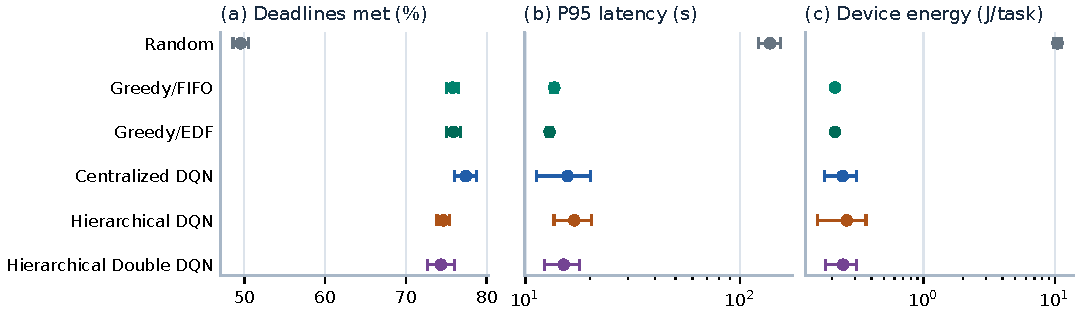
\includegraphics[width=\textwidth]{figures/final_matched_comparison.pdf}
\caption{Matched-policy comparison. Points are means and whiskers are
one sample standard deviation across training-seed means for learned
policies or across noise seeds for fixed policies. Latency and energy
use logarithmic axes.}
\label{fig:matched}
\end{figure*}

\begin{figure}[t]
\centering
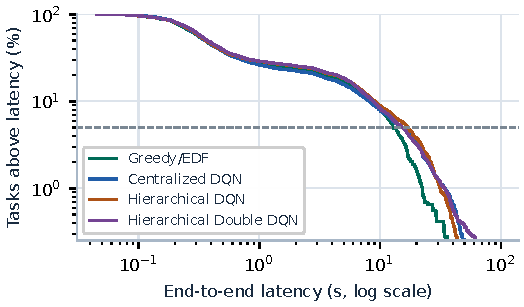
\includegraphics[width=\columnwidth]{figures/latency_tail.pdf}
\caption{Empirical latency exceedance for four policies. The dashed line
marks 5\%. The curves pool the same held-out tasks over the available
replays per policy. Table~\ref{tab:matched} averages per-replay P95 values.}
\label{fig:latency-tail}
\end{figure}

Fig.~\ref{fig:latency-tail} shows why the P95 matters. Hierarchical
DQN has a mean latency of 3.04 s and a mean per-replay P95 of
16.91 s. The high tail includes queuing, execution and transfers.
It indicates a risk for latency-sensitive IoT applications under
this compute-heavy workload and modeled contention.

\paragraph{Additional centralized control}
The primary table uses one centralized reference. As an additional
control, we evaluated the five centralized Double DQN checkpoints
under the same trace, reference topology, and five noise seeds. This
variant uses fixed EDF in the cloud and obtains $77.40\pm1.24$\%
deadline success, $13.74\pm2.08$ s P95, and $0.224\pm0.026$ J/task.
The two centralized variants have nearly identical mean success.
Centralized Double DQN has a lower mean P95, while Greedy/EDF
retains the lowest mean P95 of the evaluated policies. The
centralized control separates the choice of learning target from
the choice of information and control architecture, although
centralized and hierarchical cloud dispatch differ.

\subsection{Feedback and topology sensitivity}
To isolate feedback settings, each algorithm was evaluated with five
training seeds under each condition. Table~\ref{tab:feedback} compares
frequent updates with event-triggered updates at the checkpoint's
trained threshold. Traffic is measured per 579-task replay.

\begin{table}[t]
\centering
\caption{Coordination trade-off on the reference topology.}
\label{tab:feedback}
\footnotesize
\setlength{\tabcolsep}{4pt}
\begin{tabular}{@{}llrrr@{}}
\toprule
Learner & Mode & Success (\%) & P95 (s) & Feedback (kB) \\
\midrule
DQN & Frequent & 74.63 & 16.91 & 35.39 \\
DQN & Event 0.10 & 75.74 & 18.84 & 11.86 \\
DQN & Event 0.25 & 73.07 & 16.61 & 11.99 \\
DQN & Event 0.50 & 74.75 & 16.74 & 10.69 \\
Double DQN & Frequent & 74.33 & 15.08 & 35.13 \\
Double DQN & Event 0.10 & 74.29 & 17.00 & 11.53 \\
Double DQN & Event 0.25 & 74.95 & 17.46 & 11.09 \\
Double DQN & Event 0.50 & 74.98 & 17.80 & 10.43 \\
\bottomrule
\end{tabular}
\end{table}

At threshold 0.50, Double DQN reduces feedback traffic by 70.3\%
relative to frequent feedback, with a 0.65 percentage point increase
in observed success and a 2.72 s increase in P95. For DQN, the same
comparison reduces feedback bytes by 69.8\%, with a 0.12 point
increase in observed success and a 0.17 s decrease in P95.
These comparisons use separately trained policies and the cost
includes feedback bytes. They describe the combined effect of the
feedback mechanism and learning under that mechanism.

Four variants probe transfer to resource settings held out during
training. They increase cloud CPU, improve the device--edge link,
improve the edge--cloud link, or combine reduced CPU and link
capacity with longer propagation. Under combined stress and
frequent feedback, DQN reaches 61.73\% success and 29.42 s P95,
compared with 60.17\% and 40.41 s for Double DQN. The reference
latency ranking reverses in this condition. The matched evaluation
therefore supports conclusions tied to a workload and topology.

\subsection{Cloud scheduling with frozen upstream policies}
The cloud ablation replays each frequent-feedback checkpoint with
the learned rule selector and each fixed rule, keeping device and
edge weights, tasks and noise seeds paired. The results in
Table~\ref{tab:cloud} show the effect of switching the cloud scheduler
under the same upstream policies.

\begin{table}[t]
\centering
\caption{Cloud ablation on the reference topology.}
\label{tab:cloud}
\footnotesize
\begin{tabular}{@{}lrrrr@{}}
\toprule
 & \multicolumn{2}{c}{DQN upstream} & \multicolumn{2}{c}{Double DQN upstream} \\
Rule & Success (\%) & P95 (s) & Success (\%) & P95 (s) \\
\midrule
Learned & 74.63 & 16.91 & 74.33 & 15.08 \\
EDF & 74.65 & 16.37 & 74.24 & 15.29 \\
SPT & 75.23 & 12.26 & 74.82 & 12.36 \\
FIFO & 74.25 & 18.25 & 73.90 & 17.82 \\
\bottomrule
\end{tabular}
\end{table}

SPT gives the highest mean success and lowest mean P95 for both
upstream architectures across the five tested topologies. With the
Double DQN upstream policy on the reference, SPT reduces P95 by
2.72 s relative to its learned scheduler. All ten checkpoints
consistently select one rule whenever multiple jobs are queued, and
the corresponding fixed-rule replay reproduces their per-task
outcomes. This explains why evaluating against all three fixed rules
matters. An improvement over EDF alone could reflect the choice of a
different fixed rule. The long tail of task work and the short-service
preference in the cloud reward help explain the competitive SPT result.

\subsection{Reporting limitations}
The evaluation reports mean latency, P95 latency, deadline success,
device energy, task communication bytes, and feedback bytes; Table~\ref{tab:matched-extra}
adds the metrics not included in Table~\ref{tab:matched}. Device energy is
total modeled device CPU
and radio energy divided by the tasks in a replay, then aggregated according
to the seed aggregation described above. It excludes idle,
reception-infrastructure, retransmission, and cloud energy. Task communication bytes are data-plane payload bytes; feedback bytes are
control-plane bytes. Feedback currently does not contend with data-plane
links, so its communication cost should not be interpreted as queueing
interference.

Centralized DQN observes global state and therefore has an information
advantage over the hierarchical policies; centralized state-collection
traffic is not included in the communication accounting. The five evaluation
seeds vary simulated bandwidth and service-time noise on one chronological
test window, not five independent trace periods, and the five training seeds
provide limited evidence. The reported standard deviations are descriptive
and reflect different aggregation sources for fixed and learned policies.
